\section{Fält}
\index{elektriskt fält (E)}
\index{magnetiskt fält (H)}
För att ange nivån på det elektriska fältet (E) används enheten
''volt per meter'' (V/m).
Det magnetiska fältet (H) nivå anges i enheten ''ampere per meter'' (A/m).

Antennens uppgift är att så effektivt som möjligt omvandla den högfrekventa
strömmen i matarkabeln till en elektromagnetisk våg som utbreder sig i luften.

Den sammansatta elektromagnetiska vågen uppträder inte direkt vid antennen utan
uppstår i det som man kallar fjärrfältet.
Detta sker genom växelverkan mellan de elektriska och magnetiska fält som
utgår från antennen.
Teorierna som beskriver hur denna växelverkan fungerar är komplicerade
men det viktiga att förstå är att det finns en gräns mellan vad man
kallar fjärrfältet, längre bort från antennen och närfältet nära antennen.

\index{fjärrfält}
I fjärrfältet kan man tack vare växelverkan mellan det elektriska- och det
magnetiska fältet mäta vilket som helst av dem.
I och med att det elektromagnetiska fältet sprider ut sig över en större yta så
avtar styrkan i fältet med avståndet från antennen.
Det sammansatta elektromagnetiska fältet som passerat gränsen till fjärrfältet
avtar linjärt med avståndet, dubbleras avståndet halveras fältstyrkan.
Det spelar ingen roll om antennen är helt rundstrålande eller koncentrerar
effekten i en riktning, det elektromagnetiska fältet avtar på samma sätt.

\index{närfält}
I närfältet behöver man på grund av fältens komplicerade inbördes förhållande
mäta både det elektriska och det magnetiska fältet för att få en uppfattning
om storleken på det radiofrekventa fältet.
I antennens närhet varierar nivåerna på de olika fälten kraftigt och på vissa
punkter kan höga fältstyrkenivåer mätas upp.

Om antennen har stor utsträckning i förhållande till använd våglängd kan ibland
fjärrfältsformler användas för att överslagsmässigt beräkna fältstyrkenivå i
antennens närfält.
För kompakta antenner (t.ex. små loopar) krävs komplicerade beräkningar
med hjälp av antennsimuleringsprogram.

Beroende på den antenntyp som genererar fältet är det antingen ett elektriskt
eller magnetiskt fält som dominerar i närfältet.
Elektrisk fältdominans genereras av antenntyper som bygger på
spänningsskillnader (t.ex. dipol) och magnetisk fältdominans av antenner
med strömflöde (t.ex. små loopar).

Eftersom alla elektriska ledare kan betraktas som antenner kommer dessa att
kunna generera fält, oavsett om det är tänkt att det ska vara en antenn eller
inte.
Man bör ha detta i åtanke vid installation av matarledning till antennen för
att undvika att högfrekvent ström flyter tillbaka till stationen på utsidan av
ledningen.
Även de apparater man använder för att generera radiosignaler kan ha dålig
skärmning och därigenom leds högfrekvent ström till apparaternas utsida.

Det finns alltså en risk att fältstyrkorna kan vara betydande i närheten av
sändare och framför allt vid slutsteg med tillhörande kablage.

\section{Allmänna råd}
\index{EMF!allmänna~råd}

SSM har gett ut allmänna råd för begränsning av allmänhetens exponering
för elektromagnetiska fält SSMFS~2008:18~\cite{SSMFS2008:18}.
Syftet med råden är att skydda allmänheten från akuta
skadliga biologiska effekter vid exponering för elektromagnetiska fält.
I råden anges grundläggande begränsningar och härledda referensvärden.

\begin{quote}
	De grundläggande begränsningarna säkerställer att elektriska eller
	magnetiska fenomen som kan uppträda i kroppen inte stör funktioner i
	nervsystemet eller ger upphov till skadlig värmeutveckling.
\end{quote}

De grundläggande begränsningarna är, enligt internationella rekommendationer,
satta vid ungefär två procent av de nivåer vid vilka akuta biologiska effekter
är vetenskapligt säkerställda.

Från de grundläggande begränsningarna har härletts referensvärden som utgörs
av storheter som är mätbara utanför människokroppen.
Referensvärdena ska säkerställa att de grundläggande begränsningarna inte
överskrids.

\begin{quote}
	Om uppmätta värden överstiger referensvärdena, innebär detta inte nödvändigtvis
	att de grundläggande begränsningarna överskrids. I sådana fall gäller enligt
	dessa allmänna råd de grundläggande begränsningarna.
\end{quote}

I EU-direktivet 1999/519/EG~\cite{1999/519/EG} skrivs att i sådana fall skall det
göras en bedömning huruvida exponeringsnivån ligger under den grundläggande
begränsningen.

Referensvärdena i de allmänna råden bör inte överskridas i något område där
allmänheten kan vistas under sådana tider att begränsningarna är av betydelse.

\index{EMF!akuta biologiska effekter}
Det finns två huvudsakliga akuta biologiska effekter som kan förekomma vid
kraftig exponering för elektromagnetiska fält.
Fält med frekvens upp till cirka \qty{10}{\mega\hertz} kan om strömtätheten blir
hög i kroppen påverka det centrala nervsystemet.
Fält med frekvenser från \qty{100}{\kilo\hertz} till \qty{10}{\giga\hertz} kan
vid höga nivåer leda till en uppvärmning av kroppen.

\index{Specific Absorption Rate (SAR)}
\index{SAR}
När elektromagnetisk strålning absorberas i biologisk vävnad kan vävnaden värmas
upp.
Detta benämns ''Specific Absorption Rate'' (SAR) som mäts i enheten watt per
kilogram (\unit{\watt\per\kilo\gram}) eller milliwatt per gram
(\unit{\milli\watt\per\gram}).
SAR definieras som den energi, medelvärdesbildad över hela kroppen eller delar
av kroppen som absorberas per tidsenhet och per massenhet biologisk vävnad.

Då uppvärmningen av kroppsvävnad inte går snabbt räknar man med den medeleffekt
som under en viss tid orsakar uppvärmning.
För frekvenser mellan \qty{100}{\kilo\hertz} och \qty{10}{\giga\hertz} beräknas
SAR-värdet som medelvärdet under en sexminutersperiod.
För beräkning av SAR-värde på frekvenser överstigande \qty{10}{\giga\hertz}
hänvisas till formler för beräkning enligt SSMFS 2008:18.

Beroende på kroppens storlek i förhållande till det elektromagnetiska fältets
riktning och våglängd skapas resonansfenomen på grund av att kroppen fungerar
som en antenn.
Detta påverkar uppvärmningen på så sätt att vid frekvenser som är nära kroppens
eller kroppsdelens elektriska resonansfrekvens absorberas effekten lättare och
maximal uppvärmning uppstår.
Hos vuxna ligger denna resonansfrekvens mellan 70 och \qty{90}{\mega\hertz} om
personen står upp är och isolerad från något som kan jämföras med ett jordplan.
Även de olika kroppsdelarna kan vara resonanta.
En vuxen persons huvud är till exempel resonant vid cirka \qty{400}{\mega\hertz}.

Kroppens storlek avgör alltså vid vilken frekvens den absorberar mest effekt och
vid frekvenser över och under resonansfrekvensen så minskar uppvärmningen
orsakad av det elektromagnetiska fältet.

\index{EMF!referensvärden}
Referensvärdena tar hänsyn till detta faktum och det mest restriktiva
frekvensområdet ligger inom området 10 till \qty{400}{\mega\hertz} där effekt
lättast absorberas av kroppen.

I frekvensområdet 10 till \qty{110}{\mega\hertz} finns även en begränsning till
\qty{45}{\milli\ampere} för inducerad ström i varje extremitet i syfte att
begränsa det lokala SAR-värdet.

\largetikz{
	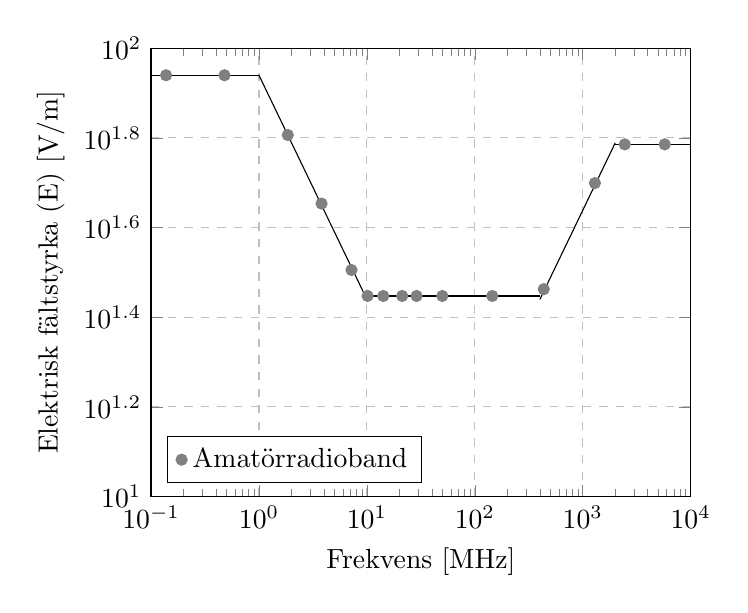
\begin{tikzpicture}
	\begin{loglogaxis}[
		xlabel={Frekvens [MHz]},
		ylabel={Elektrisk fältstyrka (E) [\unit{V/m}]},
		xmin=0.1, xmax=10000,
		ymin=10, ymax=100,
		legend pos=south west,
		grid=major, grid style=dashed,
	]

	\addplot [forget plot, domain=0.003:1, samples=10, color=black,
	]{87};

	\addplot [forget plot, domain=1:10, samples=100, color=black,
	]{8.7*10^4/(x*10^6)^(1/2)};

	\addplot [forget plot, domain=10:399.9, samples=10, color=black,
	]{28};

	\addplot [forget plot, domain=400:1999.9, samples=100, color=black,
	]{1.375*(x*10^6)^(1/2)/1000};

	\addplot [forget plot, domain=2000:10000, samples=10, color=black,
	]{61};

	\addplot[only marks, color=gray, mark=*,
		nodes near coords,
    	point meta=explicit symbolic,]
		coordinates {
		(0.1378,87)(0.479,87)(1.85,64)(3.8,45)(7.2,32)(10.15,28)(14.175,28)(21.225,28)(28.85,28)(50,28)(145,28)(435,29)(1296,50)(2450,61)(5750,61)
		};
		\legend{Amatörradioband}
	\end{loglogaxis}
	\end{tikzpicture}
}{Referensvärden för begränsning av elektriska fält på platser där allmänheten kan vistas. Amatörradioband och fältstyrkenivå angivna.}{fig:emf1}

\largetikz{
	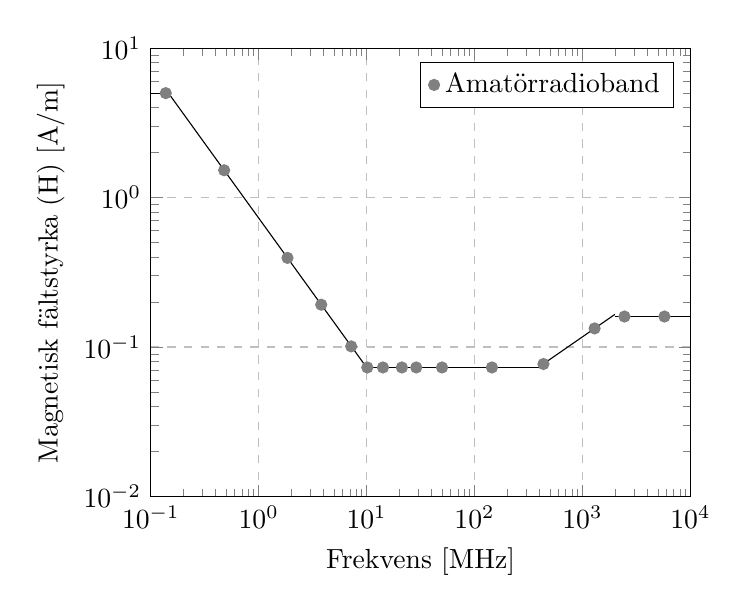
\begin{tikzpicture}
	\begin{loglogaxis}[
		xlabel={Frekvens [MHz]},
		ylabel={Magnetisk fältstyrka (H) [\unit{A/m}]},
		xmin=0.1, xmax=10000,
		ymin=0.01, ymax=10,
		legend pos=north east,
		grid=major, grid style=dashed,
	]

	\addplot [forget plot, domain=0.1:0.15, samples=10, color=black,
	]{5};

	\addplot [forget plot, domain=0.15:10, samples=100, color=black,
	]{(7.3*10^5)/(x*10^6)};

	\addplot [forget plot, domain=10:399.9, samples=10, color=black,
	]{0.073};

	\addplot [forget plot, domain=400.0:1999.9, samples=100, color=black,
	]{0.0037*(x*10^6)^(1/2)/1000};

	\addplot [forget plot, domain=2000.0:10000, samples=10, color=black,
	]{0.16};

	\addplot[only marks, color=gray, mark=*,
		nodes near coords,
    	point meta=explicit symbolic,]
		coordinates {
		(0.1378,5.0)(0.479,1.524)(1.85,0.395)(3.8,0.192)(7.2,0.101)(10.15,0.073)(14.175,0.073)(21.225,0.073)(28.85,0.073)(50,0.073)(145,0.073)(435,0.077)(1296,0.1332)(2450,0.16)(5750,0.16)
		};
		\legend{Amatörradioband}
	\end{loglogaxis}
	\end{tikzpicture}
}{Referensvärden för begränsning av magnetiska fält på platser där allmänheten kan vistas. Amatörradioband och fältstyrkenivå angivna.}{fig:emf2}

Bild~\ssaref{fig:emf1} illustrerar referensvärden för begränsning av elektriska
fält på platser där allmänheten kan vistas (100~kHz--10~GHz), med amatörband
och fältstyrkenivå angivna, till exempel \qty{10,15}{\mega\hertz} har en högsta
tillåtna elektriskt fältstyrka på \qty{28}{\volt\per\metre}.

Bild~\ssaref{fig:emf2} illustrerar referensvärden för begränsning av magnetiska
fält på platser där allmänheten kan vistas (100~kHz--10~GHz), med amatörband
och fältstyrkenivå angivna, till exempel \qty{10,15}{\mega\hertz} har en högsta
tillåtna magnetisk fältstyrka på \qty{73}{\milli\ampere\per\metre}.

\clearpage
\section{Utvärdering av EMF}
\index{EMF!utvärdering}

För att kunna utvärdera att den egna radiostationen vid sändning ger
elektromagnetiska fält som understiger referensvärdena behöver man känna till
de parametrar som är avgörande för styrkan på det elektromagnetiska fältet:

\begin{itemize}
  \item Antennens förstärkning (G).
  \item Sändningens medeleffekt (P).
  \item Transmissionsledningens förluster (k).
  \item Distansen (d).
\end{itemize}

\subsection{Antennen}
Antennen tar emot signalen från sändaren via en matningskabel och
omvandlar denna signal till en elektromagnetisk våg.
Hur effektivt antennen omvandlar signalen från sändaren kan enklast förklaras
med begreppen förstärkning eller antennvinst.

Man måste alltså känna till vilken förstärkning antennen har uttryckt i linjära
faktorer i förhållande till en isotrop antenn.

Antennförstärkning i förhållande till en isotrop antenn uttrycks vanligen i dBi.
Detta medför att en vanlig dipolantenn som används som referens för 0\,dBd har
en förstärkning på 2,15\,dBi jämfört med en isotrop antenn.

Alla värden på antennförstärkning uttryckt i dBd ska därför ökas med 2,15 för
att kunna användas i tabell~\ssaref{tab:forst} som visar förhållandet mellan
förstärkning i \unit{\decibel} och linjära faktorer.

\begin{table*}[ht]
  \begin{center}
    \begin{tabular}{|l|ccccccccccc|}
    \hline
    dB     &  0  &  1  &  2 & 2,15 &  3  &  4  &  5  &  6  &  7  &  8  &  9  \\ \hline
    G & 1,0 & 1,3 & 1,6 & 1,64 & 2,0 & 2,5 & 3,2 & 4,0 & 5,0 & 6,3 & 7,9 \\ \hline\hline
    dB     &  10  &  11  &  12  &  13  &  14  &  15  &  16  &  17  &  18  &  19  &  20 \\ \hline
    G & 10,0 & 12,6 & 15,8 & 20,0 & 25,1 & 31,6 & 39,8 & 50,1 & 63,1 & 79,4 & 100,0 \\ \hline
    \end{tabular}
    \caption{G = Antennens förstärkning i linjära faktorer}
    \label{tab:forst}
  \end{center}
\end{table*}

För en antenn med förstärkningen 7\,dBi ska alltså värdet 5,0 användas.

\subsection{Sändareffekten}
Alla SAR-värden ska beräknas som ett medelvärde under en period av sex minuter.
För att kunna utföra en beräkning av effektens medelvärde behövs utöver
PEP-effekt kännedom om de två faktorer som påverkar medeleffekten.
Faktorerna har därför betydelse för nivån på det elektromagnetiska fältet och
påverkar därigenom den genomsnittliga exponeringen för EMF.

\subsubsection{Modulationsfaktor}
\index{EMF!modulationsfaktor}
\index{modulationsfaktor}

Beroende på trafiksätt så blir medeleffekten olika.
Används FM så medför det modulationssättet att man använder max uteffekt
kontinuerligt jämfört med SSB där medeleffekten beror på hur man talar.

Tabell~\ssaref{tab:modfakt} ger de faktorer som enligt OET bulletin 65 supplement b,
\cite{OETbul65b} används i USA för att räkna ut medeleffekten på grund
av modulationsfaktorn.

\begin{table}[H]
  \begin{center}
    \begin{tabular}{lc}
	\textbf{Trafiksätt} & \textbf{Modulationsfaktor} \\ 
	\hline
	\emph{SSB} & 0,2 \\ 
	\emph{CW} & 0,4 \\ 
	\emph{SSB med processing} & 0,5 \\ 
	\emph{FM} & 1,0 \\ 
	\emph{MGM (t.ex. RTTY,PSK)} & 1,0 \\ 
	\emph{Bärvåg} & 1,0 \\ 
    \end{tabular}
    \caption{Modulationsfaktor per trafiksätt}
    \label{tab:modfakt}
  \end{center}
\end{table}

\subsubsection{Intermittensfaktor}
\index{EMF!intermittensfaktor}
\index{intermittensfaktor}

Vid vanlig amatörradioanvändning sänder man inte kontinuerligt då växling
mellan sändning och lyssning sker regelbundet.
Sänder man och tar emot lika mycket under en sexminutersperiod så blir faktorn
0,5 men om man lyssnar mycket mer och sänder sällan blir faktorn mindre.
Se tabell~\ssaref{tab:intfakt} för fler exempel.

\begin{table}[H]
  \begin{center}
    \begin{tabular}{|c|c|c|}
	\hline
	Sändning  & Mottagning & Intermittensfaktor \\
	(minuter) & (minuter)  & \\ \hline
	1 & 5 & 0,17 \\ \hline
	2 & 4 & 0,33 \\ \hline
	3 & 3 & 0,50 \\ \hline
	4 & 2 & 0,67 \\ \hline
	5 & 1 & 0,83 \\ \hline
	6 & 0 & 1,00 \\ \hline
    \end{tabular}
    \caption{Intermittensfaktor}
    \label{tab:intfakt}
  \end{center}
\end{table}

\subsubsection{Medeleffekt}
\index{EMF!medeleffekt}

För att räkna ut vilken medeleffekt som används ska man ta hänsyn
till både modulationsfaktor och intermittensfaktor enligt följande

\(\textit{Medeleffekt} = \textit{Maxeffekten} \cdot \textit{Modulationsfaktor} \cdot \textit{Intermittensfaktor}\)

\noindent\textbf{P = Medeleffekten under en sexminutersperiod}

\subsection{Kabeldämpning}
\index{EMF!kabeldämpning}

När uteffekten mäts vid sändaren och fältet genereras av effekten som
når antennen måste även den dämpning som matarledaren har vara känd.
Annars överskattas den genererade fältstyrkan.

Även här måste linjära faktorer användas.
Förlusterna i en kabel har negativa värden uttryckt i \unit{\decibel} vilket
medför att faktorerna i tabell~\ssaref{tab:feedannut} blir mindre än ett.

\begin{table*}[ht]
  \begin{center}
    \begin{tabular}{|l|c|c|c|c|c|c|c|c|c|c|c|}
	\hline
	dB & 0,0  & 0,5  & 1,0  & 1,5  & 2,0  & 2,5  & 3,0  & 3,5  & 4,0  & 4,5  & 5,0 \\ \hline
	k  & 1,00 & 0,89 & 0,79 & 0,71 & 0,63 & 0,56 & 0,50 & 0,45 & 0,40 & 0,35 & 0,32 \\ \hline
    \end{tabular}
    \caption{k = Matarkabels dämpning i linjära termer}
    \label{tab:feedannut}
  \end{center}
\end{table*}

För en kabel med dämpningen \qty{2,5}{\decibel} ska alltså värdet 0,56 användas.

\subsection{Distans}
\index{EMF!distans}

För att kunna beräkna nivån på det elektromagnetiska fältet på en utvald plats
behöver man veta distansen till den sändande antennen.

Enligt Strålsäkerhetsmyndighetens allmänna råd så bör inte referensvärdena
överskridas på platser där allmänheten vistas.
En bedömning bör därför göras över distanserna från den sändande antennen till
platser allmänheten riskerar att exponeras för elektromagnetiska fält.
\\[1ex] % layout
\noindent\textbf{d = Distansen från antennen till platsen där fältstyrkan ska bestämmas}

\subsection{Beräkning}
\index{EMF!beräkning}

Beräkning av det elektromagnetiska fältet kan med enkelhet bara
genomföras i fjärrfältet från en antenn.
I fjärrfältet vet vi sedan tidigare att man antingen kan utvärdera det
elektriska eller det magnetiska fältet.
Av denna anledning beskrivs här enbart beräkning av det elektriska fältets del av
det elektromagnetiska fältet.
Ett vedertaget avstånd från antennen där fjärrfältsberäkningar kan genomföras
är
%% \(d=\dfrac{\lambda}{6}\).
\(d=\lambda / 6\). Se tabell~\ssaref{tab:fjfltgr}.

Följande formler gäller enbart för beräkning av korrekt fältstyrka i
fjärrfältet men kan för enklare antenner användas för att uppskatta den
fältstyrka som uppträder i närfältet.

%% k7per: Where is this table referenced?
\begin{table*}[ht]
  \begin{center}
    \begin{tabular}{|l|c|c|c|c|c|c|c|c|c|c|}
	\hline
	Band [m] & 160 & 80 & 40 & 30 & 20 & 17 & 15 & 12 & 10 & 6 \\ \hline
	Fjärrfältsgräns [m] & 27 & 13 & 6,7 & 5 & 3,3 & 2,8 & 2,5 & 2 & 1,7 & 1 \\ \hline
    \end{tabular}
    \caption{Fjärrfältsgräns per band}
    \label{tab:fjfltgr}
  \end{center}
\end{table*}

\noindent\textbf{E = Det elektromagnetiska fältets storlek i fjärrfältet}

Det elektromagnetiska fältets storlek (i fjärrfältet) räknas ut från
effekten (medelvärde), antennförstärkningen, matarledningens dämpning
och avståndet enligt följande förenklade formel.
%%
\[E=\dfrac{\sqrt{30 \cdot P \cdot G \cdot k}}{d}\]
%%
Genom enkel matematik kan man då använda samma formel för att räkna
ut på vilket avstånd man genererar en viss fältstyrka.
%%
\[d=\dfrac{\sqrt{30 \cdot P \cdot G \cdot k}}{E}\]
%%
Denna beräkning är enbart relevant för huvudloben.
Fältet under antennen beräknas inte, och därför kan resultatet inte användas
för att bedöma höjd på eller säkerhetsavstånd till antenntorn.
Använd datorprogram för att få bra bedömning på hur en antenn beter sig,
särskilt med avseende på antenner med riktverkan.

\begin{exempelbox}
En riktantenn för \qty{144}{\mega\hertz} med förstärkning enligt databladet på
14,92\,dBi (31 gånger).
Max uteffekt är \qty{1000}{\watt} och trafiksättet är MGM (t.ex. RTTY, PSK) med
30~sekunders intervaller.
Den valda matarledningen har en dämpning på \qty{2,5}{\decibel} (0,56~gånger).
Avståndet från antennen till beräkningspunkten är \qty{15}{\metre}.
Vilken medelfältstyrka genererar man på ett visst avstånd från antennen?
\tcblower
\noindent
\[P_{medel} = P_{pep} \cdot k_{mod} \cdot k_{if}
= 1000 \cdot 1 \cdot 0,5 = \qty{500}{\watt}\]
\[k_{mod} = modulationsfaktor\]
\[k_{if} = intermittensfaktor\]
\[G = 31 \quad k = 0,56 \quad d = 15\]
% \[E = \dfrac{\sqrt{30 \cdot P \cdot G \cdot k}}{d}
% = \dfrac{\sqrt{30 \cdot 500 \cdot 31 \cdot 0,56}}{15}
% = \qty{34,02}{\volt\per\metre}\]
\begin{align*}
  E &= \dfrac{\sqrt{30 \cdot P \cdot G \cdot k}}{d} =\\
&= \dfrac{\sqrt{30 \cdot 500 \cdot 31 \cdot 0,56}}{15}
= \qty{34,02}{\volt\per\metre}
\end{align*}

Då referensvärdet på denna frekvens är \qty{28}{\volt\per\metre}, överskrider
amatörradiosändningen referensvärdet på detta avstånd.
\end{exempelbox}

\begin{exempelbox}
En riktantenn för \qty{144}{\mega\hertz} med förstärkning enligt databladet på
14,92\,dBi (31 gånger).
Max uteffekt är \qty{1000}{\watt} och trafiksättet är MGM (t.ex. RTTY, PSK) med
30~sekunders intervaller.
Den valda matarledningen har en dämpning på \qty{2,5}{\decibel} (0,56~gånger).
Referensvärdet för \qty{144}{\mega\hertz} är \qty{28}{\volt\per\metre}.
På vilket avstånd från antennen når man referensvärdet?
\tcblower
\noindent
\[P_{medel} = P_{pep} \cdot k_{mod} \cdot k_{if}
= 1000 \cdot 1 \cdot 0,5 = \qty{500}{\watt}\]
\[k_{mod} = \textit{modulationsfaktor}\]
\[k_{if} = \textit{intermittensfaktor}\]
\[G = 31 \quad k = 0,56 \quad E = 28\]
%% \[d = \dfrac{\sqrt{30 \cdot P \cdot G \cdot k}}{d}
%% = \dfrac{\sqrt{30 \cdot 500 \cdot 31 \cdot 0,56}}{28}
%% = \qty{18,22}{\metre}\]
\begin{align*}
  d &= \dfrac{\sqrt{30 \cdot P \cdot G \cdot k}}{d} =\\
&= \dfrac{\sqrt{30 \cdot 500 \cdot 31 \cdot 0,56}}{28}
  = \qty{18,22}{\metre}
  \end{align*}

För att följa de allmänna råden bör allmänheten inte kunna vistas i huvudloben
framför antennen på ett avstånd mindre än \qty{19}{\metre} då sändning utförs
enligt exemplet.
\end{exempelbox}

\begin{exempelbox}
En dipolantenn för \qty{3,75}{\mega\hertz} har jämfört med en isotrop antenn
förstärkningen 2,15\,dBi (cirka 1,6 gånger).
Max uteffekt är \qty{100}{\watt} och trafiksättet är SSB med normala TX/RX
intervaller.
Den valda matarledningen har en dämpning på \qty{0,5}{\decibel} (0,89 gånger).
Referensvärdet för \qty{3,75}{\mega\hertz} är \qty{45}{\volt\per\metre}.
På vilket avstånd från antennen når man referensvärdet?
\tcblower
\noindent
\[P_{medel} = P_{pep} \cdot k_{mod} \cdot k_{if}
= 100 \cdot 0,5 \cdot 0,5 = \qty{25}{\watt}\]
\[k_{mod} = modulationsfaktor\]
\[k_{if} = intermittensfaktor\]
\[G = 1,6 \quad k = 0,89 \quad E = 45\]
\[d = \dfrac{\sqrt{30 \cdot P \cdot G \cdot k}}{E} = \dfrac{\sqrt{30 \cdot 25 \cdot 1,6 \cdot 0,89}}{45}
= \qty{0,74}{\metre}\]

Här konstaterar vi att det uträknade avståndet ligger i närfältet från antennen
(inom 13~meter).
En dipol är en enklare antenntyp så vi kan anta att värdet är användbart för att
kunna utvärdera exponeringen.

För att följa de allmänna råden bör människor inte ha tillträde till nån del av
antennen närmare än \qty{0,74}{\metre} då sändning utförs.
\end{exempelbox}
